\begin{ZhChapter}

\chapter{實驗結果與分析}

\section{實驗環境與參數設計}

本研究實驗環境包含實體硬體測試平台與模擬環境平台兩部分,搭配修改後之 FruityMesh 協定,用以驗證所提出之拓樸生成與傳輸優化機制在不同環境下的效能表現。

\subsection{實體實驗平台}
實體網路建構基於 Nordic nRF52840 SoC 開發板,相關配置如表\ref{tab: 實體實驗平台配置}所示。

\begin{table}[H]
\centering
\caption{實體實驗平台配置}
\label{tab: 實體實驗平台配置}
\begin{tabular}{|c|c|}
    \hline
    項目 & 說明 \\ 
    \hline
    晶片型號 & Nordic Semiconductor nRF52840(支援 BLE 5.0) \\
    \hline
    節點數量 & 共 6 個節點(含 1 個 Sink 節點) \\
    \hline
    資料傳輸通道 & 使用 UART 作為 Log 回傳通道 \\
    \hline
    電力供應方式 & 透過 USB 供電進行情境部署 \\
    \hline
    節點與節點距離 & 小於1公尺 \\
    \hline
\end{tabular}
\end{table}

本研究所進行的實體實驗平台建置於 Nordic Semiconductor 所推出的 nRF52840-DK 開發板上,整體平台共由 6 個 nRF52840 節點組成。我們首先模擬 Sink 節點與多個子節點,再透過實際部署驗證所提出之拓樸建立機制與封包傳輸策略在真實硬體環境下的效能表現。

各節點皆搭載 Nordic 所提供之 SoftDevice BLE 堆疊,並以 FruityMesh 為基礎韌體框架進行修改與擴充。根據不同實驗目的,調整拓樸建立參數、連線策略與角色排程機制,並燒錄至各 nRF52840-DK 板上進行測試。透過 UART 紀錄各節點狀態與封包交換資訊,如圖\ref{fig: nRF52840-DK日誌紀錄},觀察節點之間的拓樸變化與網路重建過程。

實體節點部署於室內空間中,模擬感測器佈建情境。節點間距為 小於 1 公尺。所有實驗皆重複進行多次以確保結果穩定與具參考性,並與模擬平台結果進行對比分析,以佐證演算法之可行性與實用性。

\begin{figure}[H]
    \centering
    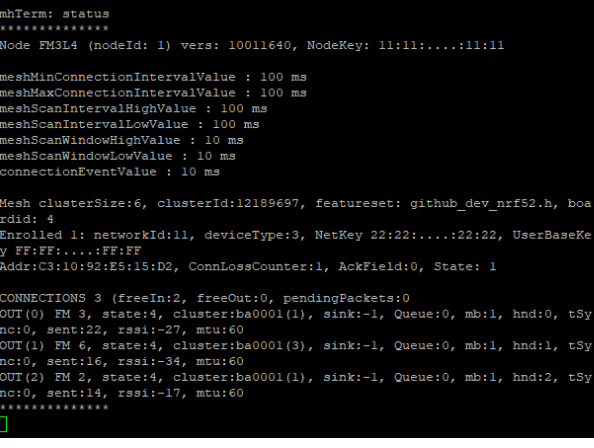
\includegraphics[width = 0.8\textwidth]{image/UART日誌紀錄.png}
    \caption{nRF52840-DK日誌紀錄}
    \label{fig: nRF52840-DK日誌紀錄}
\end{figure}

\subsection{模擬實驗平台(CheerySim)}
為進一步驗證系統在大規模節點下的可擴展性與穩定性,本研究亦使用 CheerySim 模擬器進行測試。 CherrySim 作為模擬 BLE 網路的主要工具。CherrySim 是由 FruityMesh 開發團隊所提供的官方模擬器,能夠在不需要實體硬體的情況下,模擬基於 Nordic nRF52 系列晶片及其 SoftDevice 堆疊的 BLE 節點行為。CherrySim 支援完整的連線協定模擬,包含封包交換、連線建立、訊號強度 (RSSI)、連線參數(如 CE/CI)等,並提供豐富的除錯與日誌紀錄功能。

此外,CherrySim 內建 網路狀態視覺化介面,可清楚顯示模擬過程中節點的地理分布與連線拓樸,並即時更新節點之間的連線變化。研究人員可透過該介面直觀掌握拓樸建立流程、連線演化過程與自我修復行為。

\subsubsection{模擬實驗流程}
本研究於 CherrySim 中設計三組模擬情境,分別模擬節點數為 11、21 及 31 的藍牙網路環境,每種情景分別使用3種不同seed進行模擬。每組模擬皆包含一個 Sink 節點,並配置節點4的位置為Sink點,模擬其拓樸自動生成與穩定過程,模擬觀察拓樸建立完成所需時間、自我修復機制及平均 HopsToSink 數值。

其中,11節點網狀節點配置式意圖,如圖\ref{fig: 模擬實驗11點網狀節點配置示意圖}所示,21節點網狀節點配置式意圖,如圖\ref{fig: 模擬實驗21點網狀節點配置示意圖}所示,31節點網狀節點配置式意圖,如圖\ref{fig: 模擬實驗31點網狀節點配置示意圖}所示。

\begin{figure}[H]
    \centering
    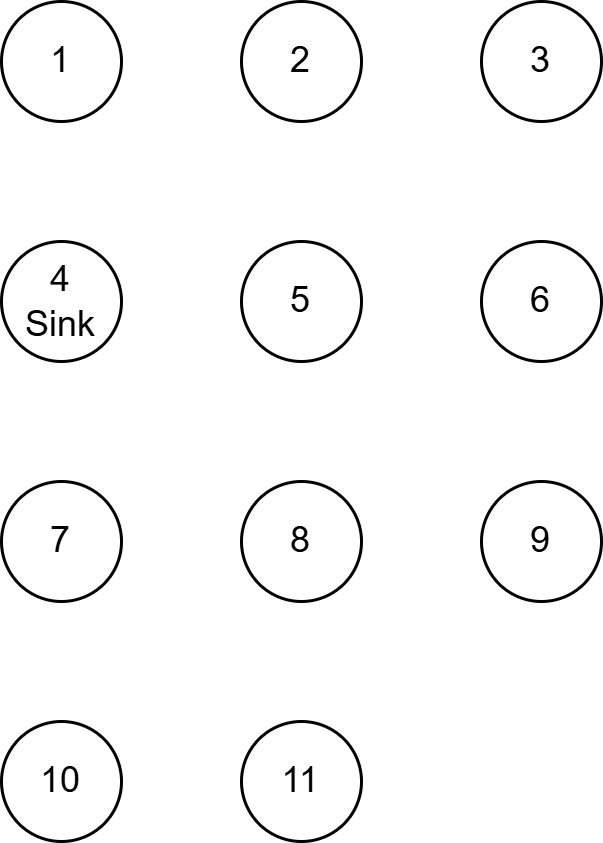
\includegraphics[width = 0.3\textwidth]{image/模擬實驗11點網狀節點配置示意圖.png}
    \caption{模擬實驗11點網狀節點配置示意圖}
    \label{fig: 模擬實驗11點網狀節點配置示意圖}
\end{figure}

\begin{figure}[H]
    \centering
    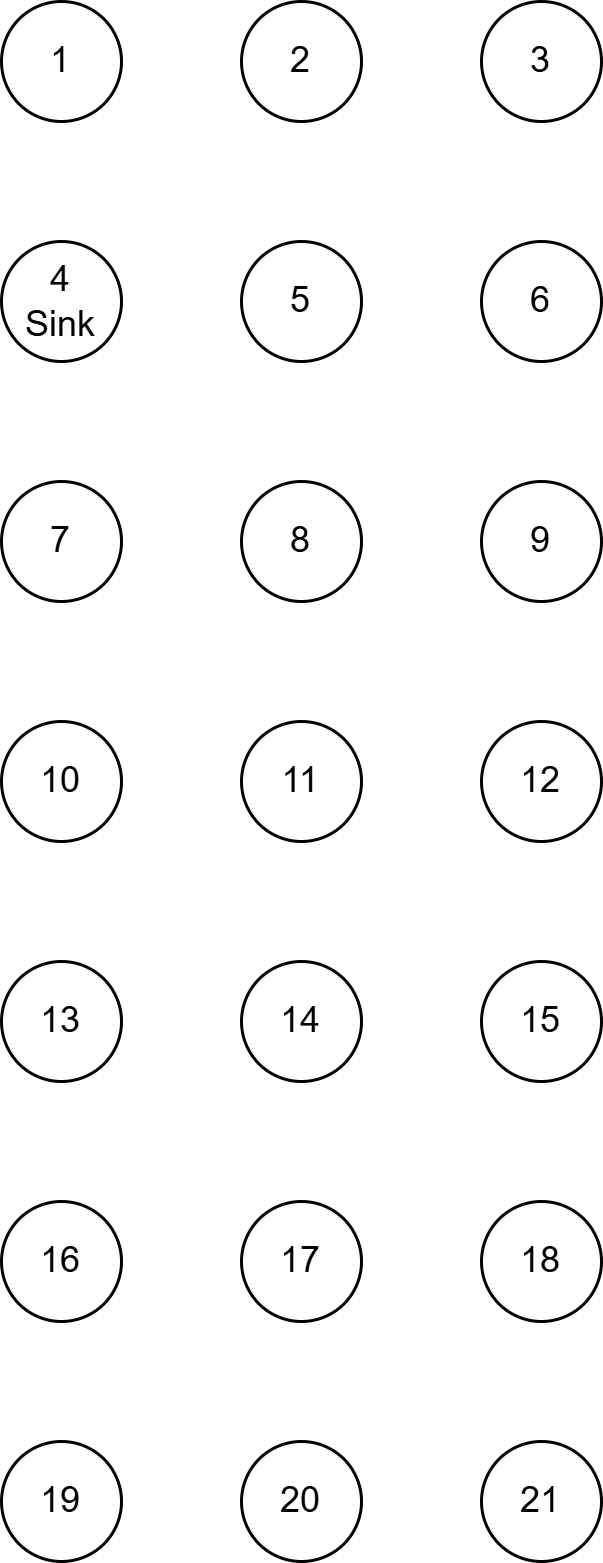
\includegraphics[width = 0.3\textwidth]{image/模擬實驗21點網狀節點配置示意圖.png}
    \caption{模擬實驗21點網狀節點配置示意圖}
    \label{fig: 模擬實驗21點網狀節點配置示意圖}
\end{figure}

\begin{figure}[H]
    \centering
    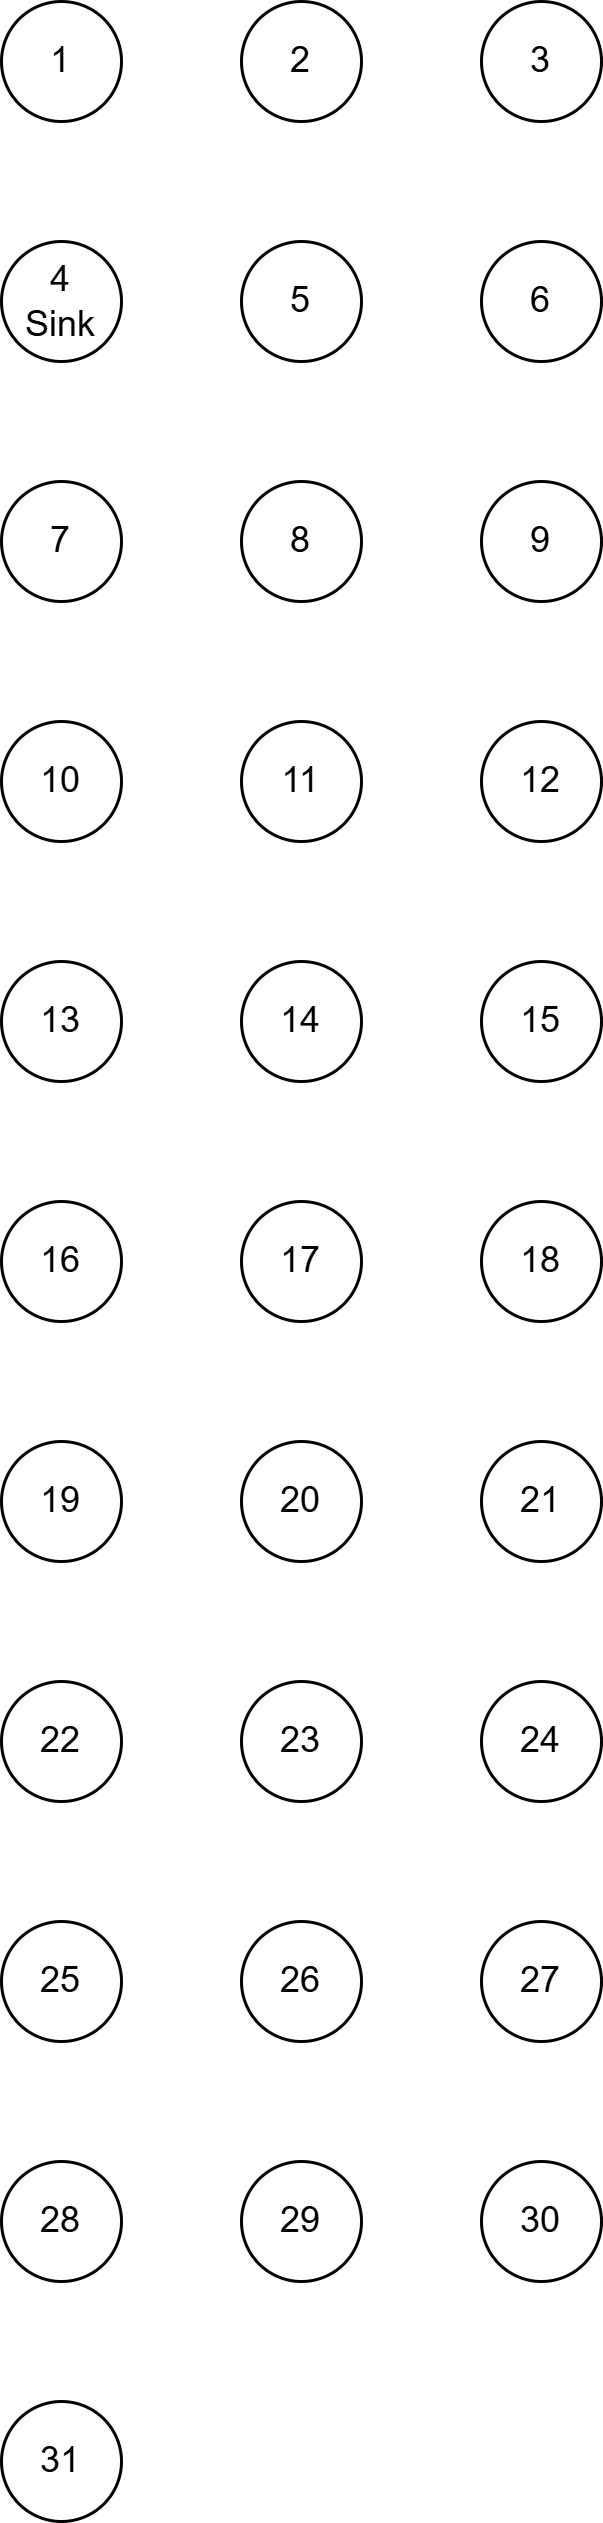
\includegraphics[width = 0.3\textwidth]{image/模擬實驗31點網狀節點配置示意圖.png}
    \caption{模擬實驗31點網狀節點配置示意圖}
    \label{fig: 模擬實驗31點網狀節點配置示意圖}
\end{figure}

\subsubsection{模擬實驗參數設定}
模擬實驗中,所有節點相關參數如表\ref{tab: 模擬實驗參數設定表}所示。表中包含Simulated Device、Node Deployment、Distance between nodes、節點數量、Sink 節點位置、Seed、Connection Interval 及 Connection Event 等參數設定。

\begin{table}[H]
    \centering
    \caption{模擬實驗參數設定表}
    \label{tab: 模擬實驗參數設定表}
    \begin{tabular}{|c|c|}
        \hline
        參數名稱 & 設定值 \\
        \hline
        Simulated Device & nRF52DK \\
        \hline
        Node Deployment & Grid \\
        \hline
        Distance between nodes & 3m \\
        \hline
        節點數量 & 11, 21, 31(including 1 sink node) \\
        \hline
        Sink 節點位置 & 節點4 \\
        \hline
        Seed & 1, 10, 100 \\
        \hline
        Connection Interval & 100 ms \\
        \hline
        Connection Event &  10 ms  \\
        \hline
    \end{tabular}
\end{table}

\section{效能評估指標}
本研究針對所提出的拓樸生成與傳輸優化機制,設計以下數項效能評估指標,以量化系統在不同模擬情境下的表現。

\subsection{拓樸建立時間}
拓樸建立時間是指節點成功建立 Mesh 拓樸所需的時間。此指標反映系統在節點加入網路時的效率,時間越短表示系統越能快速適應新節點,具備更佳的擴展性與部署靈活性,如\ref{eq: TopologyEstablishmentTime}式所示。

\begin{equation}
\label{eq: TopologyEstablishmentTime}
\text{TopologyEstablishmentTime} = Topology_{finish} - Topology_{init}
\end{equation}
其中:
\begin{itemize}
    \item $Topology_{finish}$ 為拓樸建立完成的時間點。
    \item $Topology_{init}$ 為拓樸建立開始的時間點。
\end{itemize}

\subsection{自我修復時間}
自我修復時間指的是節點在斷線後,能夠重新加入網路並恢復傳輸功能所需的時間。此指標評估網路面對節點失效或路徑中斷時的容錯能力與恢復效率,能顯示出 Mesh 結構的穩定性,如\ref{eq: SelfHealingTime}式所示。

\begin{equation}
\label{eq: SelfHealingTime}
\text{SelfHealingTime} = Topology_{finish} - Node_{disconnection}
\end{equation}

其中:
\begin{itemize}
    \item $Topology_{finish}$ 為拓樸建立完成的時間點。
    \item $Node_{disconnection}$ 為節點斷線的時間點。
\end{itemize}

\subsection{平均 HopsToSink 數值}
平均 HopsToSink 表示封包從任意節點傳送至 Sink 節點所需的平均跳數。此數值越低代表網路拓樸越扁平,資料傳輸的路徑越短,能有效降低延遲並提升整體效率,如\ref{eq: AvgHopsToSink}式所示。

\begin{equation}
\label{eq: AvgHopsToSink}
\text{AvgHopsToSink} = \frac{\sum HopsToSink}{N_{nodes}}
\end{equation}

其中:
\begin{itemize}
    \item $\sum HopsToSink$ 為所有節點到 Sink 節點的跳數總和。
    \item $N_{nodes}$ 為網路中節點的總數,不包含Sink節點。
\end{itemize}

\subsection{平均封包傳輸延遲}
此指標衡量封包從來源節點產生到 Sink 節點成功接收所經歷的時間總和,反映網路整體的即時性與處理能力,此值越低,代表網路回應時間越短、傳輸效率越高。如\ref{eq: AvgPacketDelay}式所示。
\begin{equation}
\label{eq: AvgPacketDelay}
\text{AvgPacketDelay} = \frac{\sum Delay_{end-to-end}}{\sum N_{sink\_received\_packet}}
\end{equation}

其中:
\begin{itemize}
    \item $\sum Delay_{end-to-end}$ 為所有成功接收封包從來源節點產生至 Sink 節點接收之總延遲時間。
    \item $\sum N_{sink\_received\_packet}$ 為所有成功接收封包的總數。
\end{itemize}

\subsection{平均封包抵達率}

平均抵達率(Average Packet Delivery Ratio, PDR)表示成功接收封包的總數,佔來源節點原本應發送封包總數的比例,當網路品質下降或傳輸負載過高時,PDR 會明顯降低,如\ref{eq: AvgPDR}式所示。

\begin{equation}
\label{eq: AvgPDR}
\text{AveragePDR} = \frac{\sum N_{sink\_received\_packet}}{\sum N_{source\_send\_packet}} \times 100\%
\end{equation}

其中:
\begin{itemize}
    \item $\sum N_{sink\_received\_packet}$ 為所有成功接收的封包數量。
    \item $\sum N_{source\_send\_packet}$ 為所有來源節點發送的封包數量。
\end{itemize}

\subsection{平均封包重傳率(Average Retransmission Rate)}

平均重傳率衡量封包在網路中被重複傳送的比例,反映網路壅塞或角色衝突導致的傳輸效率問題,重傳率越低,代表網路越穩定、資源使用效率越高,如\ref{eq: AvgRetransmissionRate1}式及\ref{eq: AvgRetransmissionRate2}式。

\begin{equation}
\label{eq: AvgRetransmissionRate1}
\text{AvgRetransmissionRate} = \frac{\sum RetransmissionPacket}{\sum Conn_{expect\_send\_packet}} \times 100\%
\end{equation}

\begin{equation}
\label{eq: AvgRetransmissionRate2}
\sum RetransmissionPacket = \sum Conn_{actual\_send\_packet} - \sum Conn_{expect\_send\_packet}
\end{equation}

其中:
\begin{itemize}
    \item $\sum Conn_{expect\_send\_packet}$ 為所有節點預期應發送的封包數量(包含中繼節點轉傳的封包)。
    \item $\sum Conn_{actual\_send\_packet}$ 為實際發送的封包總數(包含重傳)。
    \item $\sum RetransmissionPacket$ 為實際重傳封包的總數。
\end{itemize}

\section{實驗結果與分析}
本研究針對所提出的拓樸生成與傳輸優化機制,進行實體與模擬環境下的效能評估。以下分別呈現實體實驗平台與模擬平台的實驗結果,並針對各項效能指標進行分析。

\subsection{模擬提出之網路拓樸建立}
模擬實驗中,使用 CheerySim 平台進行三組不同節點數量的拓樸建立測試。每組模擬均包含一個 Sink 點,並配置節點4位置當作Sink節點。實驗結果顯示,所提出的網路拓樸演算法能夠確保Sink節點,也就是節點4的位置,位於拓樸的根節點,其中,圖\ref{fig: 模擬實驗11點seed=1}、\ref{fig: 模擬實驗11點seed=10}及\ref{fig: 模擬實驗11點seed=100}所示,分別表示節點數量為11點時,Seed分別為1、10、100的模擬結果;圖\ref{fig: 模擬實驗21點seed=1}、\ref{fig: 模擬實驗21點seed=10}及\ref{fig: 模擬實驗21點seed=100}所示,分別表示節點數量為21點時,Seed分別為1、10、100的模擬結果;圖\ref{fig: 模擬實驗31點seed=1}、\ref{fig: 模擬實驗31點seed=10}及\ref{fig: 模擬實驗31點seed=100}所示,分別表示節點數量為31點時,Seed分別為1、10、100的模擬結果。

\begin{figure}[H]
    \centering
    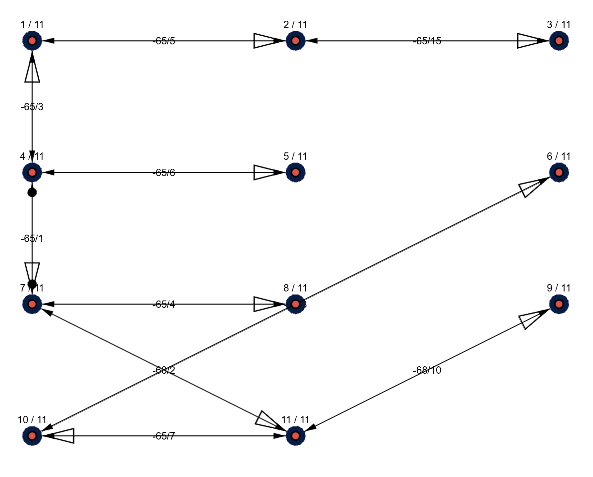
\includegraphics[width = 0.6\textwidth]{image/模擬實驗11點seed=1.png}
    \caption{模擬節點數量=11點,Seed=1}
    \label{fig: 模擬實驗11點seed=1}
\end{figure}

\begin{figure}[H]
    \centering
    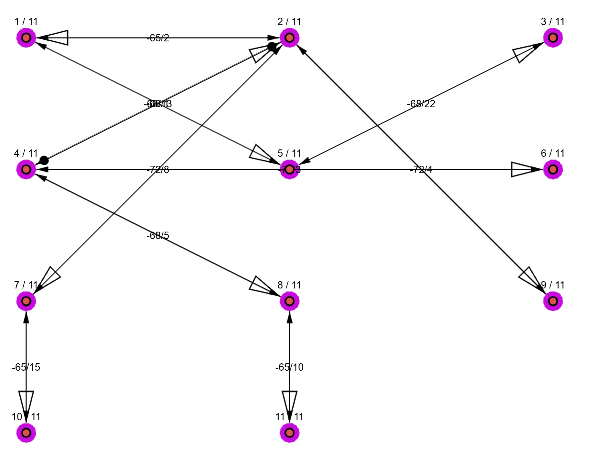
\includegraphics[width = 0.6\textwidth]{image/模擬實驗11點seed=10.png}
    \caption{模擬節點數量=11點,Seed=10}
    \label{fig: 模擬實驗11點seed=10}
\end{figure}

\begin{figure}[H]
    \centering
    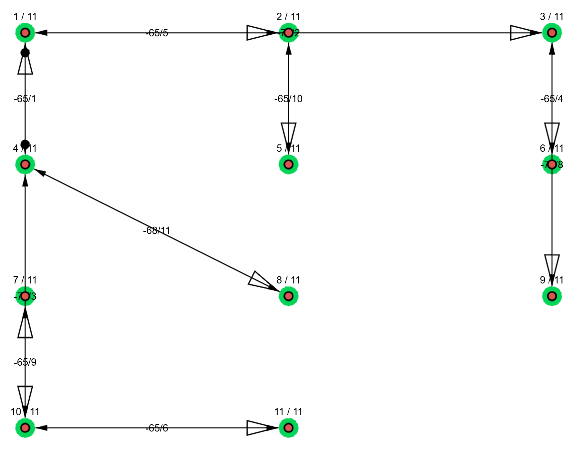
\includegraphics[width = 0.6\textwidth]{image/模擬實驗11點seed=100.png}
    \caption{模擬節點數量=11點,Seed=100}
    \label{fig: 模擬實驗11點seed=100}
\end{figure}

\begin{figure}[H]
    \centering
    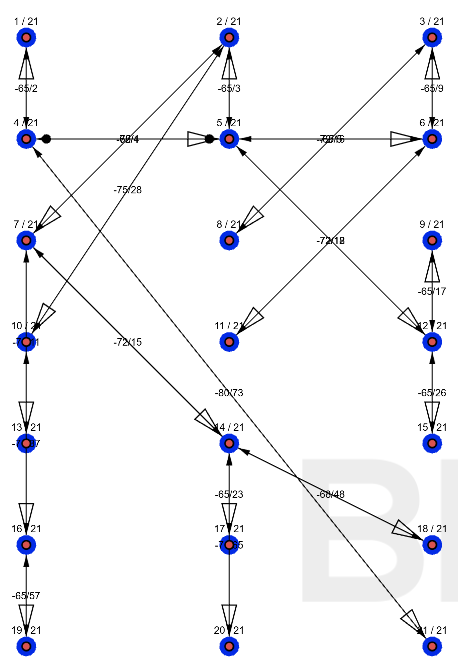
\includegraphics[width = 0.6\textwidth]{image/模擬實驗21點seed=1.png}
    \caption{模擬節點數量=21點,Seed=1}
    \label{fig: 模擬實驗21點seed=1}
\end{figure}

\begin{figure}[H]
    \centering
    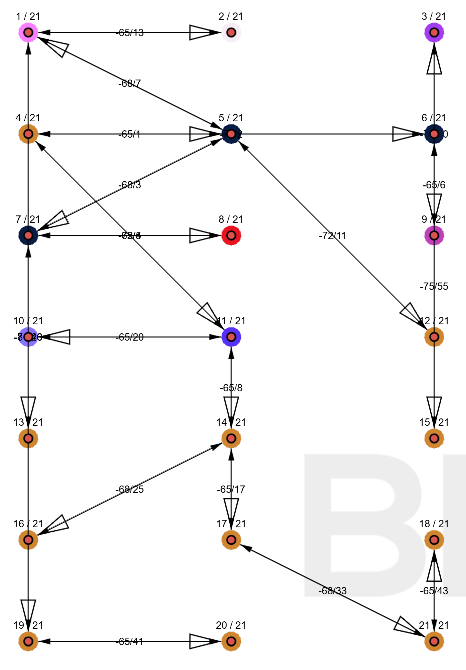
\includegraphics[width = 0.6\textwidth]{image/模擬實驗21點seed=10.png}
    \caption{模擬節點數量=21點,Seed=10}
    \label{fig: 模擬實驗21點seed=10}
\end{figure}

\begin{figure}[H]
    \centering
    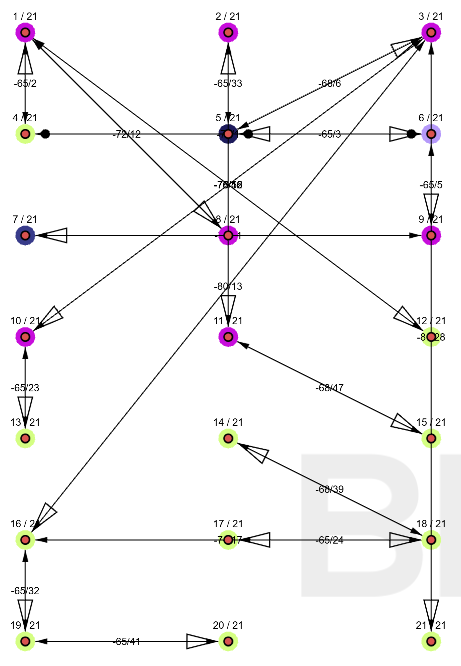
\includegraphics[width = 0.6\textwidth]{image/模擬實驗21點seed=100.png}
    \caption{模擬節點數量=21點,Seed=100}
    \label{fig: 模擬實驗21點seed=100}
\end{figure}

\begin{figure}[H]
    \centering
    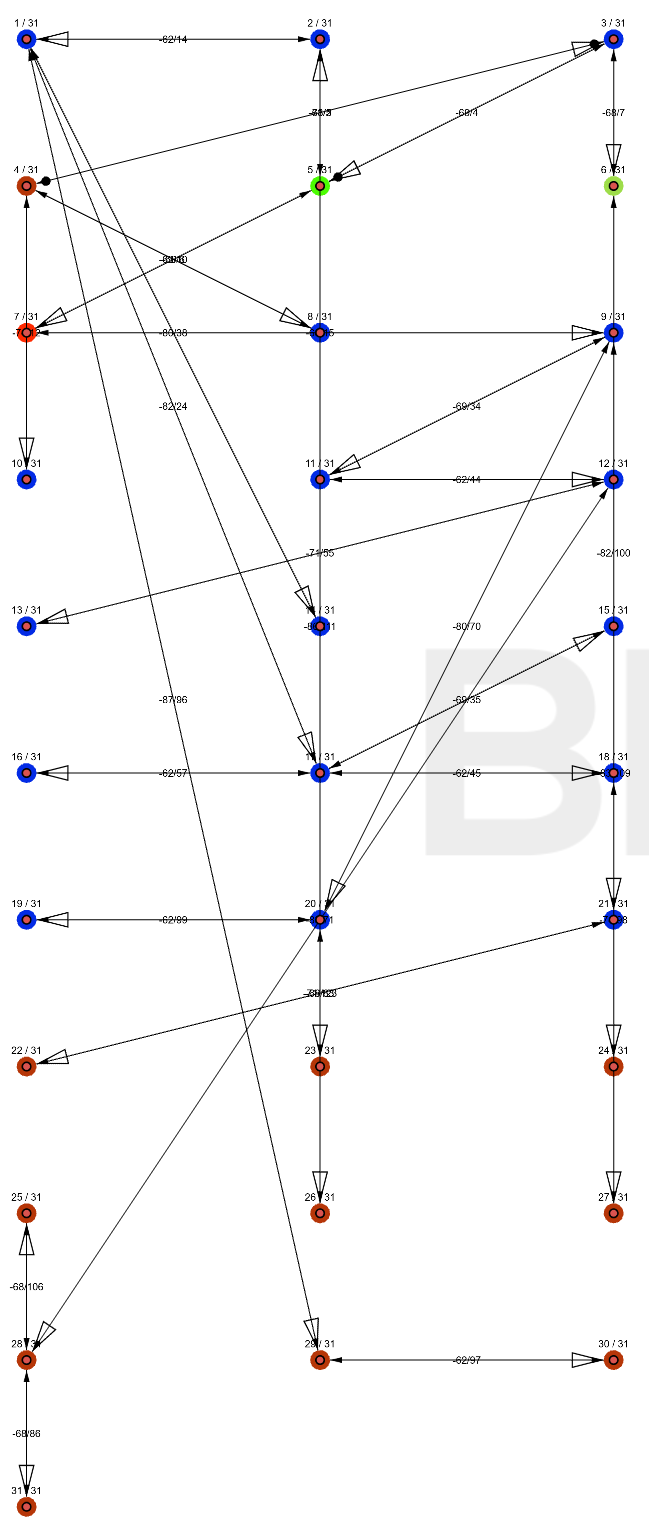
\includegraphics[width = 0.6\textwidth]{image/模擬實驗31點seed=1.png}
    \caption{模擬節點數量=31點,Seed=1}
    \label{fig: 模擬實驗31點seed=1}
\end{figure}

\begin{figure}[H]
    \centering
    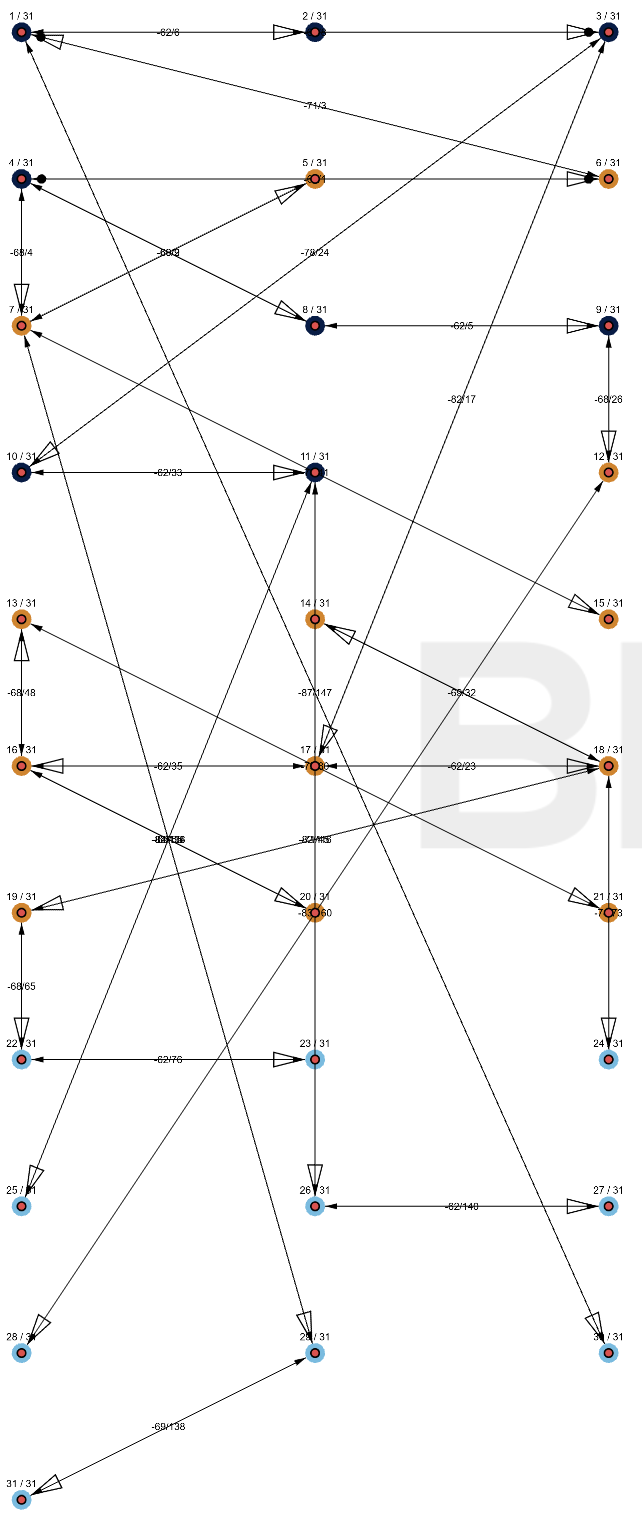
\includegraphics[width = 0.6\textwidth]{image/模擬實驗31點seed=10.png}
    \caption{模擬節點數量=31點,Seed=10}
    \label{fig: 模擬實驗31點seed=10}
\end{figure}

\begin{figure}[H]
    \centering
    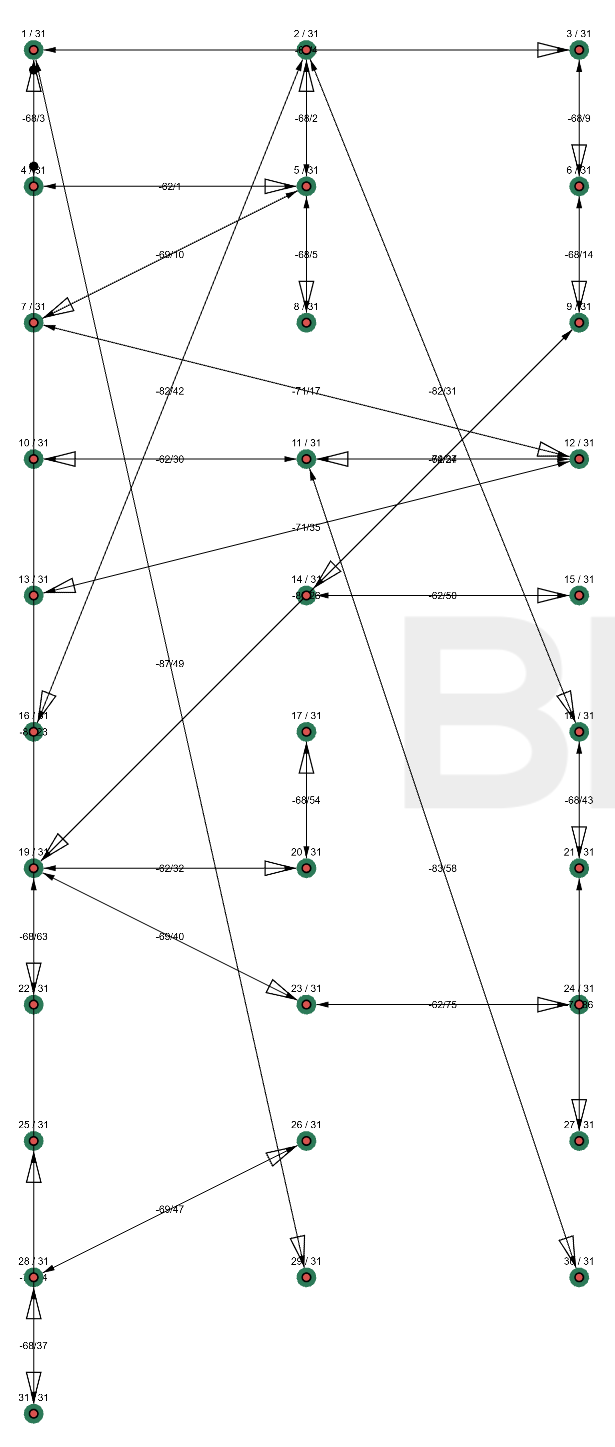
\includegraphics[width = 0.6\textwidth]{image/模擬實驗31點seed=100.png}
    \caption{節點數量=31點,Seed=100}
    \label{fig: 模擬實驗31點seed=100}
\end{figure}

\subsection{模擬提出之網路拓樸Sink 節點斷線後拓樸重建機制}
模擬實驗中,會將 Sink 節點斷線後,Mesh系統能夠自動重新建立拓樸並確保 Sink 節點仍然是根節點。分別以節點數量11、21及31實驗10次,圖\ref{fig: 模擬實驗11點sink斷線後連回}、\ref{fig: 模擬實驗21點sink斷線後連回}及\ref{fig: 模擬實驗31點sink斷線後連回}分別顯示了節點數量為11、21及31時,Sink節點(節點位置4)斷線後重新連線後的結果。可以觀察到,即使在 Sink 節點斷線後,Mesh系統仍能恢復並保持Sink節點(節點位置4)在拓樸的根節點。

\begin{figure}[H]
    \centering
    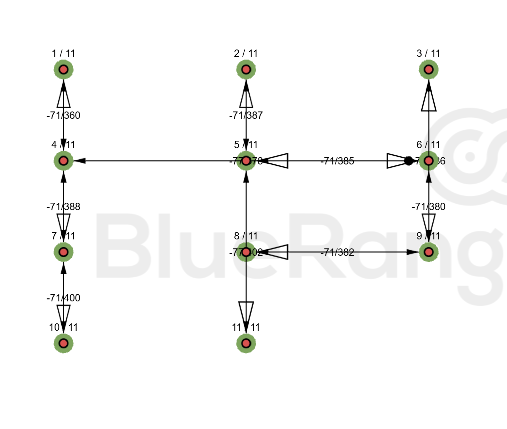
\includegraphics[width = 0.8\textwidth]{image/模擬實驗11點sink斷線後連回.png}
    \caption{模擬實驗11點sink斷線後連回結果}
    \label{fig: 模擬實驗11點sink斷線後連回}
\end{figure}

\begin{figure}[H]
    \centering
    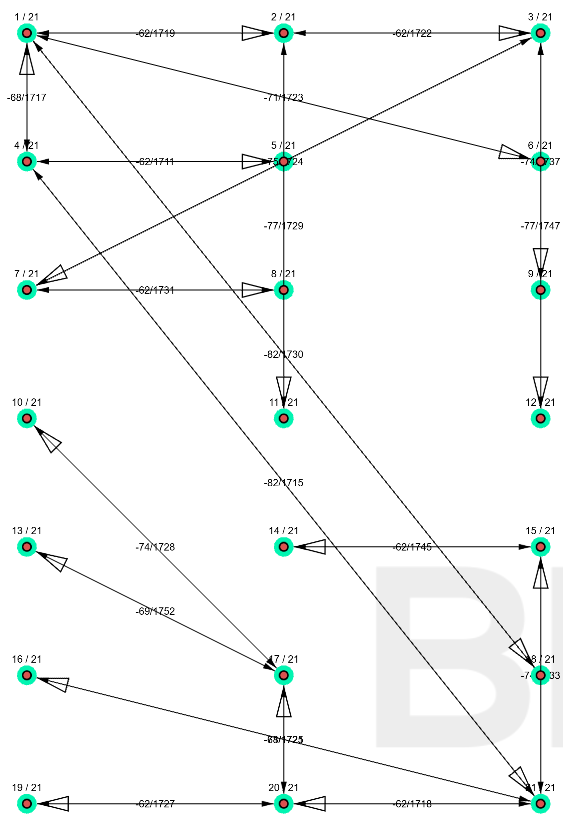
\includegraphics[width = 0.8\textwidth]{image/模擬實驗21點sink斷線後連回.png}
    \caption{模擬實驗21點sink斷線後連回結果}
    \label{fig: 模擬實驗21點sink斷線後連回}
\end{figure}

\begin{figure}[H]
    \centering
    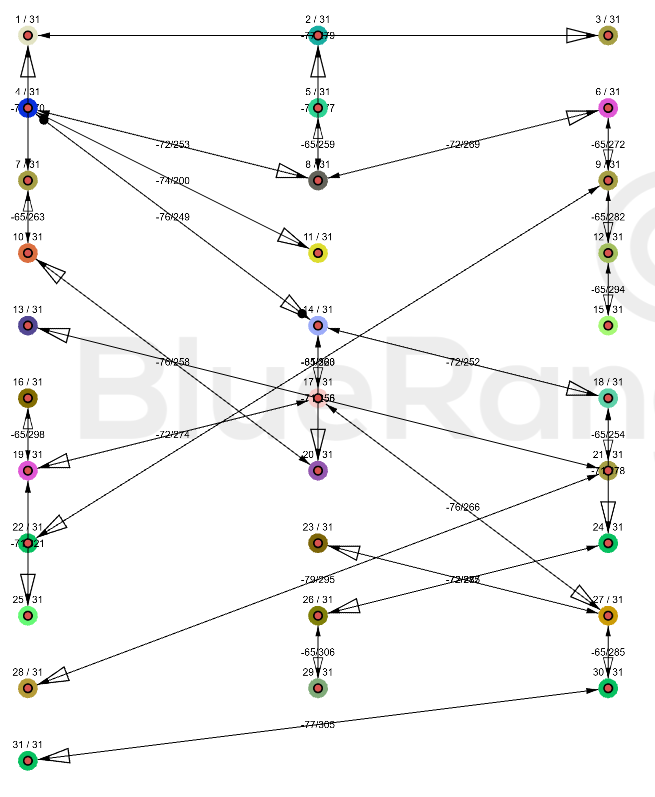
\includegraphics[width = 0.8\textwidth]{image/模擬實驗31點sink斷線後連回.png}
    \caption{模擬實驗31點sink斷線後連回結果}
    \label{fig: 模擬實驗31點sink斷線後連回}
\end{figure}


\subsection{模擬節點重啟後之拓樸重建時間分析}
在本研究中,為驗證所提出機制於節點重啟(reset)後的拓樸重建效率,設計了不同網路規模下的模擬實驗。實驗分別針對節點總數為 11、21 及 31 的網路拓樸進行,並比較兩種節點類型的重啟情境,分別為 Sink 節點(根節點)與非 Sink 節點(一般中繼節點或邊緣節點)。

每一種網路規模與節點類型情境下,皆進行 100 次重啟測試,記錄節點自啟動至成功連入 Mesh 網路所需之時間,並據此計算其平均連線時間與標準差。透過大量重複實驗,能更準確評估系統在拓樸變動下的穩定性與恢復能力,並觀察不同節點角色對 Mesh 重建效率的影響。

本實驗分別於 11 點、21 點與 31 點之網路拓樸規模下,針對 Sink 節點與非 Sink 節點進行模擬測試。每組情境皆重複執行 100 次實驗,統計其 Mesh 成功建立所需的平均時間與標準差,結果如圖 \ref{fig: 節點重啟後之拓樸重建時間分析} 所示。

\begin{figure}[H]
    \centering
    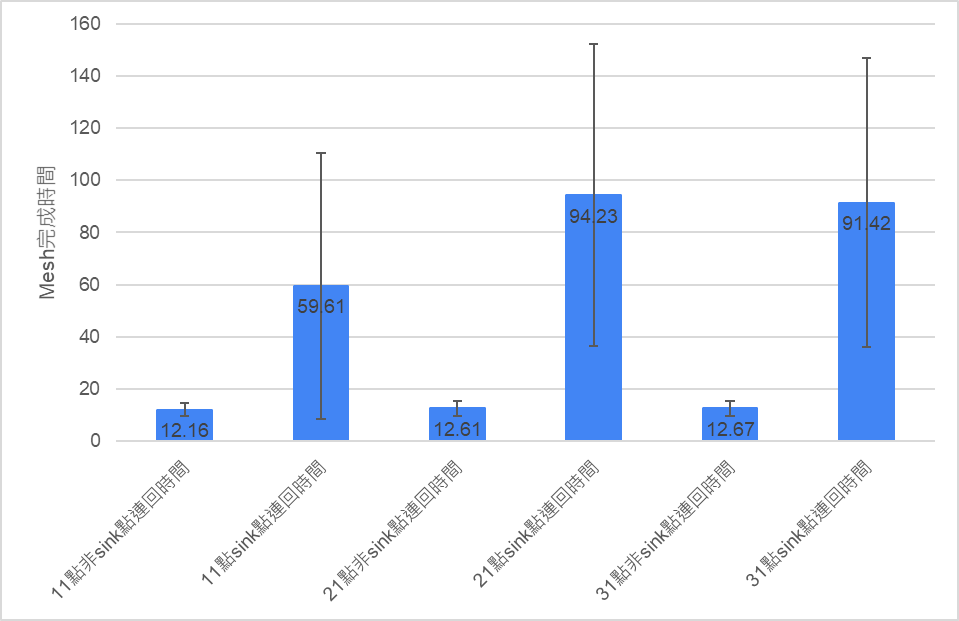
\includegraphics[width = 0.8\textwidth]{image/節點重啟後之拓樸重建時間分析.png}
    \caption{模擬節點重啟後之拓樸重建時間分析}
    \label{fig: 節點重啟後之拓樸重建時間分析}
\end{figure}

從實驗結果可觀察到,在三種網路規模下,非 Sink 節點的重啟連線平均時間皆維持在約 12.1~12.7 秒之間,且標準差相對較小(約 2.3~3.0),顯示其連線行為穩定且具一致性。而相較之下,Sink 節點的重啟平均時間顯著較高,分別為 59.61 秒(11 點)、94.23 秒(21 點)與 91.42 秒(31 點),且標準差也明顯較大(達 50~57),顯示在重建根節點角色與拓樸過程中,其恢復行為具有較高的變異性與延遲風險。

此現象可歸因於 Sink 節點在拓樸中需重新扮演根節點角色,並建立樹狀結構的主幹連線路徑,因此重啟後需耗費較多時間進行握手、選擇路徑與節點重連。此外,實驗亦證實所提出之拓樸修復機制能在重啟後正確辨識 Sink 節點並讓其重新成為 Mesh 拓樸的根節點,保持網路層級的一致性與穩定性。

\subsection{模擬不同節點數與隨機環境下拓樸平衡性分析}
本節實驗針對原生 FruityMesh 與本研究所提出之修改後演算法在拓樸平衡性上的表現進行比較。拓樸平衡性的衡量方式以節點連向 Sink 節點所需跳數(HopsToSink)作為評估依據,平均值與最大值越低表示拓樸越平衡、傳輸路徑越有效率。

為驗證演算法於不同隨機環境下之穩定性,實驗設計採用三組隨機種子,seed = 1、10、100,並分別在節點數為 11、21 與 31 的情境中進行測試,觀察各版本之平均 HopsToSink 與最大 HopsToSink 指標,如表\ref{tab: Seed = 1時的平均 HopsToSink 與最大 HopsToSink}、\ref{tab: Seed = 10時的平均 HopsToSink 與最大 HopsToSink}及\ref{tab: Seed = 100時的平均 HopsToSink 與最大 HopsToSink}。

從實驗數據觀察,節點數為 11 點時,本研究提出之演算法在三組 Seed 中皆能有效降低平均 HopsToSink 數值。例如,Seed = 10 時原生 FruityMesh 的平均跳數為 3.27,而修改演算法僅為 1.91,最大跳數也從 5 降至 4,顯示修改機制能使節點更有效地連接至 Sink 節點,拓樸結構更為平衡。

在 21 點節點數下,Seed = 10 與 Seed = 100 的實驗中亦呈現類似趨勢。修改演算法可使平均 HopsToSink 明顯下降(例如 Seed = 10 時由 4.14 降為 2.43),最大跳數亦由 7 降為 5。此結果顯示在中等節點密度下,修改後之選擇連線機制具備更強的拓樸優化能力。

針對 31 點情境,雖然在 Seed = 1 的實驗中平均跳數略升(由 4.35 增為 4.55),但在其他兩組 Seed(Seed = 10 與 100)中,修改演算法仍可降低平均 HopsToSink(由 4.03 降為 3.65;由 5.10 降為 3.39),顯示本機制在高節點密度下仍能維持穩定之優化效果,並有效壓低拓樸樹的深度與最大跳數。

整體而言,修改後的演算法在大多數情境下均能降低節點到 Sink 的平均跳數,證實其在拓樸平衡性與傳輸效率上的改進成效。尤其在節點數越多的情境中,平均跳數的改善更為明顯。

\begin{table}[H]
    \centering
    \caption{模擬Seed = 1時的平均 HopsToSink 與最大 HopsToSink}
    \label{tab: Seed = 1時的平均 HopsToSink 與最大 HopsToSink}
    \begin{tabular}{|c|c|c|c|}
        \hline
          &節點數量 & 平均 HopsToSink & 最大 HopsToSink \\
        \hline
        原生 FruityMesh & 11 & 2.55 & 5 \\
        \hline
        本研究所提出之演算法 & 11 & 1.82 & 3 \\
        \hline
        原生 FruityMesh & 21 & 2.86 & 6 \\
        \hline
        本研究所提出之演算法 & 21 & 2.90 & 7 \\
        \hline
        原生 FruityMesh & 31 & 4.35 & 8 \\
        \hline
        本研究所提出之演算法 & 31 & 4.55 & 8 \\
        \hline
    \end{tabular}
\end{table}

\begin{table}[H]
    \centering
    \caption{模擬Seed = 10時的平均 HopsToSink 與最大 HopsToSink}
    \label{tab: Seed = 10時的平均 HopsToSink 與最大 HopsToSink}
    \begin{tabular}{|c|c|c|c|}
        \hline
          &節點數量 & 平均 HopsToSink & 最大 HopsToSink \\
        \hline
        原生 FruityMesh & 11 & 3.27 & 5 \\
        \hline
        本研究所提出之演算法 & 11 & 1.91 & 4 \\
        \hline
        原生 FruityMesh & 21 & 4.14 & 7 \\
        \hline
        本研究所提出之演算法 & 21 & 2.43 & 5 \\
        \hline
        原生 FruityMesh & 31 & 4.03 & 7 \\
        \hline
        本研究所提出之演算法 & 31 & 3.65 & 7 \\
        \hline
    \end{tabular}
\end{table}

\begin{table}[H]
    \centering
    \caption{模擬Seed = 100時的平均 HopsToSink 與最大 HopsToSink}
    \label{tab: Seed = 100時的平均 HopsToSink 與最大 HopsToSink}
    \begin{tabular}{|c|c|c|c|}
        \hline
          &節點數量 & 平均 HopsToSink & 最大 HopsToSink \\
        \hline
        原生 FruityMesh & 11 & 2.64 & 5 \\
        \hline
        本研究所提出之演算法 & 11 & 1.82 & 3 \\
        \hline
        原生 FruityMesh & 21 & 3.05 & 6 \\
        \hline
        本研究所提出之演算法 & 21 & 3.48 & 6 \\
        \hline
        原生 FruityMesh & 31 & 5.10 & 9 \\
        \hline
        本研究所提出之演算法 & 31 & 3.39 & 6 \\
        \hline
    \end{tabular}
\end{table}

\subsection{實作提出之網路拓樸建立}
實體實驗中,使用 6塊 Nordic nRF52840-DK 開發板進行小規模拓樸建立測試,表\ref{tab: 實作提出之網路拓樸建立參數設定}為相關參數設定。每個節點均配置為 FruityMesh 協定堆疊,並透過 UART 進行日誌紀錄。

\begin{table}[H]
    \centering
    \caption{實作提出之網路拓樸建立參數設定}
    \label{tab: 實作提出之網路拓樸建立參數設定}
    \begin{tabular}{|c|c|}
        \hline
        參數名稱 & 設定值 \\
        \hline
        節點數量 & 6(包含1個Sink節點) \\
        \hline
        Sink 節點編號 & 1 / 5 \\
        \hline
        Connection Interval & 100 ms \\
        \hline
        Connection Event & 10 ms \\
        \hline
    \end{tabular}
\end{table}

\subsubsection{實作初始化拓樸中Sink點之Root角色實驗}
為驗證本研究所提出的拓樸建立機制是否能正確地將指定之 Sink 節點設定為整個 BLE Mesh 網路的 Root(根節點),本實驗設計兩組不同的節點配置情境進行觀察。每組實驗均包含 6 個 nRF52840 節點,其中僅指定其中一節點為 Sink,其餘皆設定為 Static 類型,並透過 UART 回傳每個節點之拓樸連線資訊,以視覺化方式呈現網路結構。

在第一組實驗中,節點編號為 1(nodeId = 1)者被指定為 Sink 節點,初始化完成後之網路拓樸如圖 \ref{fig: 實作sink=1初始化拓樸圖} 所示。從拓樸圖可觀察到,所有節點皆透過多層結構連接至節點 1,且未出現多個中心節點或分離子網情形,顯示該節點成功成為整體 Mesh 的根節點。

\begin{figure}[H]
    \centering
    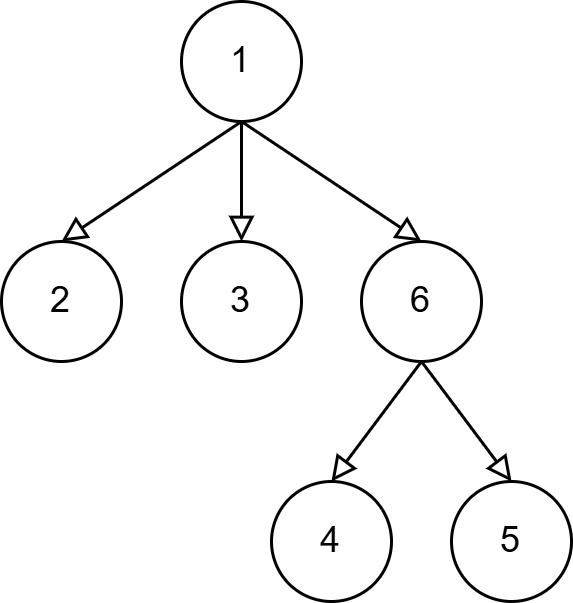
\includegraphics[width = 0.3\textwidth]{image/實作sink=1初始化拓樸圖.jpg}
    \caption{實作sink=1初始化拓樸圖}
    \label{fig: 實作sink=1初始化拓樸圖}
\end{figure}

於第二組實驗中,改由節點 5(nodeId = 5)作為 Sink,其他節點仍為 Static。初始化後之連線關係如圖 4.Y 所示,同樣可觀察到所有節點皆以節點 5 為樞紐,逐層建立向外擴展之拓樸,符合樹狀結構設計原則,Sink 成功成為網路中心。

\begin{figure}[H]
    \centering
    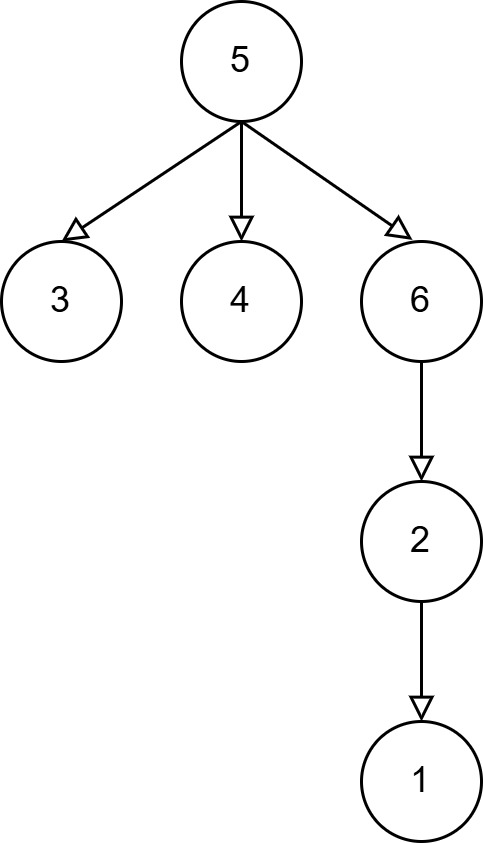
\includegraphics[width = 0.3\textwidth]{image/實作sink=5初始化拓樸圖.jpg}
    \caption{實作sink=5初始化拓樸圖}
    \label{fig: 實作sink=5初始化拓樸圖}
\end{figure}

此兩組實驗皆證實,本研究所實作之拓樸建立演算法在初始化階段能正確識別 Sink 節點,並將其設為網路的 Root。即使在不同位置指定 Sink 節點(如節點 1 或 5),皆可以達到以 Sink 為中心之拓樸結構。

\subsubsection{實作重啟拓樸中Sink點之Root角色實驗}
在本實驗中,針對已建立之 BLE Mesh 拓樸進行節點重啟測試,以驗證系統在節點重啟後能否正確恢復拓樸結構並保持 Sink 節點的 Root 角色。實驗中,分別將節點 1 及 節點 5 設定為 Sink 節點,並透過 UART 日誌紀錄其連線狀態。

在節點 1 重啟後,系統能夠自動重新建立拓樸,並確保節點 1 仍然是整個 Mesh 網路的根節點。圖 \ref{fig: 實作sink=1重啟拓樸圖} 顯示了重啟後的拓樸結構,從中可見所有節點仍然以節點 1 為根節點,完成拓樸建立。

\begin{figure}[H]
    \centering
    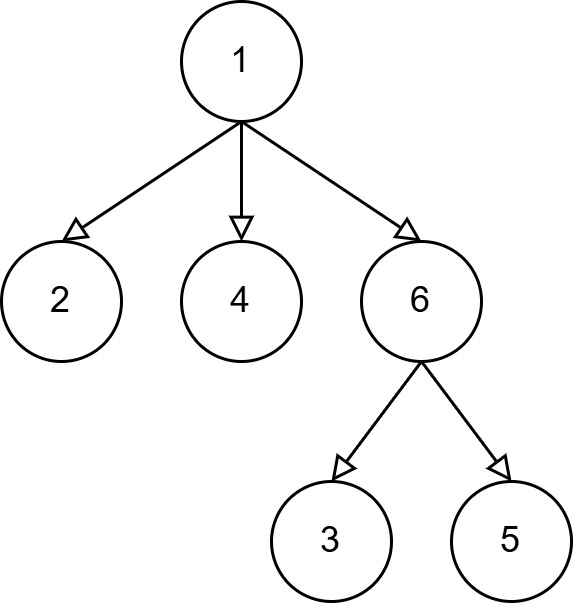
\includegraphics[width = 0.3\textwidth]{image/實作sink=1重啟拓樸圖.jpg}
    \caption{實作sink=1重啟拓樸圖}
    \label{fig: 實作sink=1重啟拓樸圖}
\end{figure}

同樣地,當節點 5 重啟後,系統亦能正確識別其為 Sink 節點,並重新建立拓樸結構。圖 \ref{fig: 實作sink=5重啟拓樸圖} 顯示了節點 5 重啟後的拓樸結構,所有節點仍然以節點 5 為根節點,完成拓樸建立。

\begin{figure}[H]
    \centering
    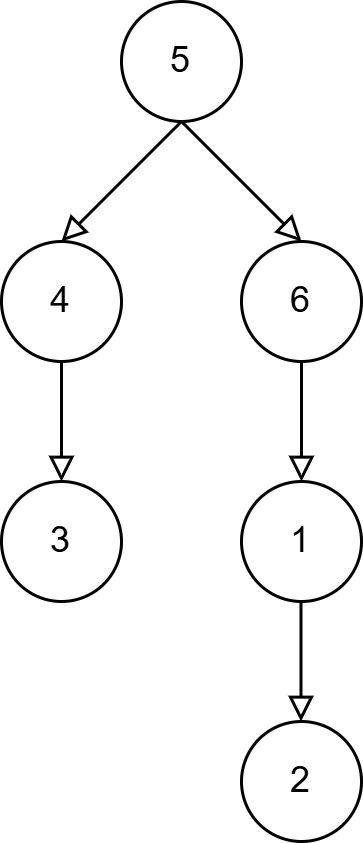
\includegraphics[width = 0.3\textwidth]{image/實作sink=5重啟拓樸圖.jpg}
    \caption{實作sink=5重啟拓樸圖}
    \label{fig: 實作sink=5重啟拓樸圖}
\end{figure}

\section{調整 Connection Interval 對網路穩定性的影響評估}
(Todo)

\end{ZhChapter}